\documentclass{cards}

\begin{document}
	\pagestyle{empty}

%   Vertical space correction for longer titles
%   \cardtitle{\vspace{-5mm}MUCH LONGER TITLE}

	\begin{tikzpicture}
		\cardtypePerLongRest
		\cardtitle{Pact Negotiation}
		\cardcontent{Following a long rest, you can...}{Book of Binding p3}
		\cardprice{$\infty$}
		\cardborder
	\end{tikzpicture}
	\hpad
	\begin{tikzpicture}
		\cardtypePerRest
		\cardtitle{Renegotiation}
		\cardcontent{Once per day when you finish a short rest, you can choose to perform the ritual of binding again to renegotiate any of the bargains you have made earlier in the day. This allows you to expel a bound vestige early and bind another in its place. When you choose to renegotiate your pacts, you can expel as many vestiges as you wish, and bind a number of vestiges whose combined level is no more than half your binder level (rounded up).}{Book of Binding p3}
		\cardprice{$\infty$}
		\cardborder
	\end{tikzpicture}
	\hpad
	\begin{tikzpicture}
		\cardtypePerTurn
		\cardtitle{Suppress Sign}
		\cardcontent{When you make a good pact with a vestige, you can use a bonus action to suppress or display the physical sign of that vestige.}{Book of Binding p3}
		\cardprice{B}
		\cardborder
	\end{tikzpicture}
	\hpad
	\begin{tikzpicture}
		\cardtypePerRest
		\cardtitle{}
		\cardcontent{}{}
		\cardprice{}
		\cardborder
	\end{tikzpicture}

	\vpad
	\begin{tikzpicture}
		\cardtypePerTurn
		\cardtitle{}
		\cardcontent{}{}
		\cardprice{}
		\cardborder
	\end{tikzpicture}
	\hpad
	\begin{tikzpicture}
		\cardtypePerTurn
		\cardtitle{}
		\cardcontent{}{}
		\cardprice{}
		\cardborder
	\end{tikzpicture}
	\hpad
	\begin{tikzpicture}
		\cardtypePerRest
		\cardtitle{}
		\cardcontent{}{}
		\cardprice{}
		\cardborder
	\end{tikzpicture}
	\hpad
	\begin{tikzpicture}
		\cardtypePerTurn
		\cardtitle{}
		\cardcontent{}{}
		\cardprice{}
		\cardborder
	\end{tikzpicture}

	\vpad
	\begin{tikzpicture}
		\cardtypePerTurn
		\cardtitle{}
		\cardcontent{}{}
		\cardprice{}
		\cardborder
	\end{tikzpicture}
	\hpad
	\begin{tikzpicture}
		\cardtypePerTurn
		\cardtitle{}
		\cardcontent{}{}
		\cardprice{}
		\cardborder
	\end{tikzpicture}
	\hpad
	\begin{tikzpicture}
		\cardtypePerTurn
		\cardtitle{}
		\cardcontent{}{}
		\cardprice{}
		\cardborder
	\end{tikzpicture}
	\hpad
	\begin{tikzpicture}
		\cardtypePerTurn
		\cardtitle{}
		\cardcontent{}{}
		\cardprice{}
		\cardborder
	\end{tikzpicture}

	\vpad
	\begin{tikzpicture}
		\cardtypePerTurn
		\cardtitle{}
		\cardcontent{}{}
		\cardprice{}
		\cardborder
	\end{tikzpicture}
	\hpad
	\begin{tikzpicture}
		\cardtypePerTurn
		\cardtitle{}
		\cardcontent{}{}
		\cardprice{}
		\cardborder
	\end{tikzpicture}
	\hpad
	\begin{tikzpicture}
		\cardtypePerTurn
		\cardtitle{}
		\cardcontent{}{}
		\cardprice{}
		\cardborder
	\end{tikzpicture}
	\hpad
	\begin{tikzpicture}
		\cardtypePerTurn
		\cardtitle{}
		\cardcontent{}{}
		\cardprice{}
		\cardborder
	\end{tikzpicture}

\end{document}
